% Chapter 5: Conclusion

\chapter{Conclusion}
\label{sec:conclusion}

Plasma irregularities in the \(F\)-region ionosphere have been observed for decades.  However, despite extensive data sets collected over these years, supprisingly little is known about these irregularities, especially at small scales.  This is in part due to the complex and turbulent nature of the ionosphere, particularly in the polar regions, but also due to some of the inherent limitations in traditional observation techniques which can make it very challenging to identify exactly what processes are operational.  In this Chapter, we summarize the results that have previously been discussed in Chapters \ref{sec:paper1}--\ref{sec:paper3}, shown in Figure \ref{fig:conclusion}, and consider what overarching conclusions can be derived from them.  Additionally, Section \ref{sec:futurework} will provide recommendations for future research which will help answer some of the still outstanding questions and further our understanding of small-scale polar \(F\)-region plasma irregularities.

\section{Summary of Results and Conclusions}
\label{sec:summary}

In the polar caps, backscatter is often observed at nighttime even when background plasma density is low and propagation conditions are traditionally thought to be too poor for FAIs to be observed with HF radar.  This implies an additional source of nighttime plasma density that is not easily accounted for by models.  Frequent polar patches that propagate from the dayside to the nightside could be the source of this additional density.  The requirements for confirming this hypotheis will be detailed further in Section \ref{sec:futurework}.

\begin{figure}
  \includegraphics[width=\textwidth]{conclusion.pdf}
  \caption[Irregularity production factors]{Summary of the main conclusions in this thesis as to what factors most effect pasma irregularity production.}
  \label{fig:conclusion}
\end{figure}

Nighttime observations of FAIs is also higher with a positive IMF By component.  This could be due to the control that the By component exerts over ionospheric convection patterns.  In a convectional two-cell convection pattern with predominantly negative IMF Bz, the plasma flows antisunward from dayside to nightside across the terminator.  In this arrangement, the plasma flow, \(\vec{V}_E\), and the density gradient, \(\vec{G}\), are antiparallel, the least favorable orientation for GDI growth.  However, with a significant IMF By component, the orientation of the convection cells rotates such that plasma no longer convects directly antisunward, creating a situation where GDI is more favorable and plasma structures can develop more readily.  Additionally, an IMF By component can contribute to the formation of polar patches by creating convection perturbations that separate high density patches from the daytime reservoir, as described in Section \ref{sec:lit_patches}.  In this way, the IMF By component may be indirectly responsible for the increased observation of backscatter.  If patch occurrence increases, it can contribute to the nighttime background density, as described above, which can improve propagation conditions so that FAIs can be observed by 
HF radars.

In addition to simply providing additional background density so nighttime propagation conditions are sufficient for the radar to observe FAIs, polar patches can contribute to plasma irregularity formation directly by providing background density gradients for GDI to be operational on.  This raises the important question of exactly how and where plasma structures form around polar patches.  Observations have long suggested there is asymmetry in plasma structuring surrounding polar patches \citep{Weber1984,Milan2002b,Koustov2012}, but the results presented in Chapter \ref{sec:paper2} suggest that production may also be anisotropic, Figure \ref{fig:conclusion}.  Asymmetry and anisotropy are independent such that the plasma structures can exhibit either of them independently or both or neither.

The plasma drift and wavevector directions influence the asymmetry that is observed surrounding polar patches.  The direction that the patch is drifting relative to its elongation direction impacts the orientations of \(\vec{G}\) and \(\vec{V}_E\) and controls the GDI growth rate.  This also creates the asymmetry between the different edges of the patch because as the gradient direction changes, the irregularity growth rate changes.  Additionally, linear theory predicts that irregularity growth is anisotropic, so the orientation of the patch relative to the radar can also impact the observed irregularities.  In the \(F\) region, the GDI growth rate is highest for wavevectors perpendicular to the gradient, \(\vec{G}\).  Although plasma waves can occur in all directions, a SuperDARN radar will only observe waves who's wavevectors are parallel to a radar beam.  Because of this, irregularities as well as structure asymmetry are most likely to be maximized if the radar's boresight is parallel to the structure's elongation, Figure \ref{fig:conclusion}.

Plasma irregularities are observed most often close to the terminator.  This is likely due to the presence of a very large density gradient between high density solar illuminated plasma on the dayside and low density plasma on the nightside.  The large background gradient promotes irregularity production through GDI.  In addition, if a SuperDARN radar itself is positioned close to the terminator, it is observing the density gradient along its boresight, Figure \ref{fig:conclusion}.  As discussed above, if small-scale irregularity growth is directionally dependent, this is additionally the optimal orientation from which to observe the plasma structures, leading to increased echo occurrence.


\section{Recommendations for Future Research on \(F\) Region Plasma Irregularities}
\label{sec:futurework}

Although much progress has been made in understanding small-scale plasma structuring and HF radar observations, many of the results presented in this thesis give rise to further questions that must be addressed.

In Chapter \ref{sec:paper1}, the occurence of radar backscatter durring nighttime in the polar cap was found to be much higher than expected \citep{Bristow2011}, particularly given that raytracing simulations predict that the orthagonality condition is rarely met and therefore there should be little to no backscatter, Figure \ref{fig:month_avg_occ}.  The proposed hypothesis to explain this discreperency is that polar patches, which are not typically well represented by ionospheric density models, occur frequently in the nighttime \(F\) region and, on average, enhance the background plasma density enough that propagation conditions are sufficient for HF radar backscatter to regularly be observed.  Experimental surveys of polar patches have shown low occurrence at nighttimes, however the occurrence of patches and their intensity increase at equinox, which is where frequent nighttime backscatter is predominantly observed \citep{Rodger1996}.  The expected signature in the radar data from this kind of senario would be a night with a series of isolate ``patches'' of backscatter.  An example of such an event was presented, Figure \ref{fig:patchy_example}, but it is unknown how often events like this occur.  Additionally, the intensity and size of a patch nessesary to cause the radar beam to refract sufficiently must be established, possibly through further use of raytracing simulations with customizable density profiles.

One of the major drawbacks to linear GDI theory is that it inherently assumes long wavelengths, which means if the \(F\) region, it technically should not be directly applicable to decameter-scale irregularities measured by HF radars.  Generally, it is assumed that some form of turbulent cascade connects plasma structures of different scale sizes in the ionosphere such that predictions made at large scales can still be applied to decameter-scale observations \citep{Tsunoda1988}.  This helps explain some of the observations of asymmetry around polar patches, which is predicted at large scales but often observed at decameter scales with radars \citep[e.g.][]{Weber1984,Milan2002b,Koustov2012}.  This asymmetry was also confirmed in the GDI growth rate from the results shown in Chapter \ref{sec:paper2}.  However, these results also predicted anisotropy in the growth rate, which is more challenging to confirm from small-scale irregularity obsersavtions, although some evidence of such has been provided in Chapter \ref{sec:paper3}.  It may be possible to further the theoretical understanding of GDI at small scales by developing a three dimentional picture of it using kinetic theory.  \citet{Basu1995} developed such a formulation for a specific geometry throughout all altitudes within the ionosphere, but expanding this to general vector directions would not be trivial, mathematically.  However, modeling irregularity growth with such a formulation may be helpful to understand how plasma structures develop at such small scales.

The results presented in Chapter \ref{sec:paper3} could also be improved with a more extensive data set.  The event chosen for analysis in that study was in 2011 and was selected on the basis of good data coverage from both RISR-N and RKN and a strong density gradient being apparent in the overlapping FoV.  Since then, RISR-C has been deployed with a FoV just south of RISR-N (Figure \ref{fig:isrmap}) such that observations between both radars can be coordinated and they can act as a single instrument with a FoV twice as large.  This allows a polar patch to be tracked over a longer distance and more individual data points to be captured.  Additionally, specific modes can be utilized that give a much finner grid of RISR beams, allowing measurements to be made closer together and smaller scale gradients to be be considered.  The downside to these modes is that it takes longer for each set of measurements to be made, so the temporal cadence decreases.  However, the required integration time for an ISR decreases if the background ionospheric density is higher, so the the temporal resolution can improve for measurements taken durring summer or daytime.  Another advantage to the RISR-N/RISR-C locations is that the SuperDARN radars at Clyde River (CLY) and Inuvik (INV) (Figure \ref{fig:superdarnmap}), both of which share at least part of the RISR-N/RISR-C FoV, but observe it from different directions.  This presents an unique opportunity to further investigate the directional dependence of small-scale irregularities by observing the differences in backscatter observed from the same scattering volume at different directions.  Although straight forward in theory, this experiment would most likely prove nontrivial in practice.  Backscatter tends to be limited to the statistical high occurrence band shown in Figure \ref{fig:month_avg_occ}, and at least with INV, this band probably occurs at closer ranges than where the FoV overlaps other radars, so coincident backscatter is probably rare.  The probability of backscatter being observed is better when the background density is within the range where propagation conditions are most favorable, when the ionosphere is sunlit.  Additionally, it is advantageous to choose a time when the occurrence of backscatter is statistically high.  Based on results from Chapter \ref{sec:paper1}, the best time for such an experiment would therefore be daytime durring an equinox month.

In Chapter \ref{sec:paper3}, both the occurrence and power of radar backscatter are used as proxies to indicate the ``amount'' of irregularities that exist in the ionosphere.  However, the trends from these quantities are rarely in good agreement, giving rise to the question what, if anything, does each of them indicate about the plasma structuring in the ionosphere.  The factors that control each need to be isolated, but this is nontrivial.  Echo occurrence generally agrees with the linear GDI theory predictions but echo power only does for relatively low power.  Irregularities may develop as predicted by linear GDI theory when their amplitudes are small but other nonlinear processes may impact larger density perturbations, such as shear-driven instabilities \citep{Gondarenko2006} or multistep processes \citep{Carlson2012}.  By the radar equation, the power returned should be proportional to the product of the background density and fractional density, squared, Equation \ref{eqn:fractional_density}.  However, there is no general consensus on what controls the fractional density in the \(F\) region, although it has been suggested that it is either constant or a function of convection speed, \(V_E\) \citep{Kustov1988,Haldoupis1990,Makarevich2014b}.  In Chapter \ref{sec:paper3}, we additionally propose it may be a function of the instability growth rate, \(\gamma\).  Because ground based radars are so often used to investigate ionospheric irregularities, this is an important issue to resolve to develop an accurate picture of how radar observations relate to plasma irregularities.

\bibliographystyle{uafthesis}
\bibliography{references}
